\section{Epitope-structure audit: three AND-gate antigens have no experimental structure (AlphaFold DB + RCSB PDB)}
The previous audits showed the AND-gate antigens are invisible to L1000
perturbation assays and mostly to the small-molecule pharmacopeia. A CAR,
however, does not need a drug-binding pocket; it needs an epitope. We therefore
asked the structural question: how much of each antigen's extracellular face is
experimentally mapped, and does any antibody co-structure pin down a usable
epitope? For 201 genes (99 gated antigens, 98 random surfaceome background,
4 approved CAR-T references) we pulled the reviewed human UniProtKB entry
(topology, signal, GPI lipidation, PDB cross-references), the AlphaFold DB
monomer model (per-residue pLDDT), and RCSB PDB polymer-entity descriptions
(1,286 entries) for every entry overlapping the annotated ectodomain. 82
genes had no UniProt membrane topology at all and were analysed separately;
the annotated set is 54 gated, 61 background, 4 references.

\paragraph{Positive control (3 of 4 pass).} The approved CAR-T antigens show
antibody-fragment co-structures (CD19 (3), ERBB2 (24), FOLR1 (0), TNFRSF17 (7)). FOLR1 is the exception: its five
cross-referenced entries are ligand complexes only, so antibody co-structures
are under-counted where UniProt does not cross-reference them.

\paragraph{Result.} Gated antigens are \emph{not} structurally worse off than
the random surfaceome background: any-ectodomain-structure rates 0.63 versus
0.44 ($p=0.1$), antibody co-structure rates 0.30 versus 0.21 ($p=0.68$), and
median experimental ectodomain coverage 0.64 versus 0.00 ($p=0.069$). The
AlphaFold-confidence difference (median pLDDT 87 versus 84, $p=0.029$) is
small. The fifth invisibility axis is therefore \emph{antigen-specific}, not
gate-wide. Within the AND gate (Table~\ref{tab:epitope}) it splits the seven
targets: MSLN is epitope-rich (5 antibody co-structures, full coverage), CA12
is covered with one Fab co-structure (6RPS), PSCA is covered but has no
antibody complex, and 3 of the seven --- CLDN18, CLDN6, and SLC39A6 ---
have \emph{no} experimental ectodomain structure at all; for these, epitope
choice currently rests on prediction alone (and SLC39A6's predicted ectodomain
is mostly low-confidence, pLDDT 51). This is a concrete, falsifiable gap: the
first experimental structures of these three ectodomains will directly confirm
or refute the epitopes the gate design assumes.

\begin{table}[h]\centering\footnotesize
\caption{Structural evidence for the seven AND-gate antigens: UniProt topology,
ectodomain length, median AlphaFold pLDDT, experimental coverage, antibody
co-structures in the PDB.}\label{tab:epitope}
\begin{tabular}{p{1.6cm}p{1.7cm}p{1.2cm}p{1.2cm}p{1.4cm}p{1.6cm}}
\hline
Antigen & topology & ectodomain aa & pLDDT & exp. coverage & ab co-structures \\ \hline
CLDN18 & multi-pass & 84 & 72 & 0.00 & 0 \\
CLDN6 & multi-pass & 76 & 83 & 0.00 & 0 \\
SLC39A6 & multi-pass & 362 & 51 & 0.00 & 0 \\
CA9 & single-pass & 377 & 80 & 0.70 & 0 \\
CA12 & single-pass & 277 & 95 & 0.95 & 1 \\
PSCA & GPI & 72 & 94 & 1.00 & 0 \\
MSLN & GPI & 303 & 87 & 1.00 & 5 \\
\hline\end{tabular}\end{table}

\begin{figure}[h]\centering
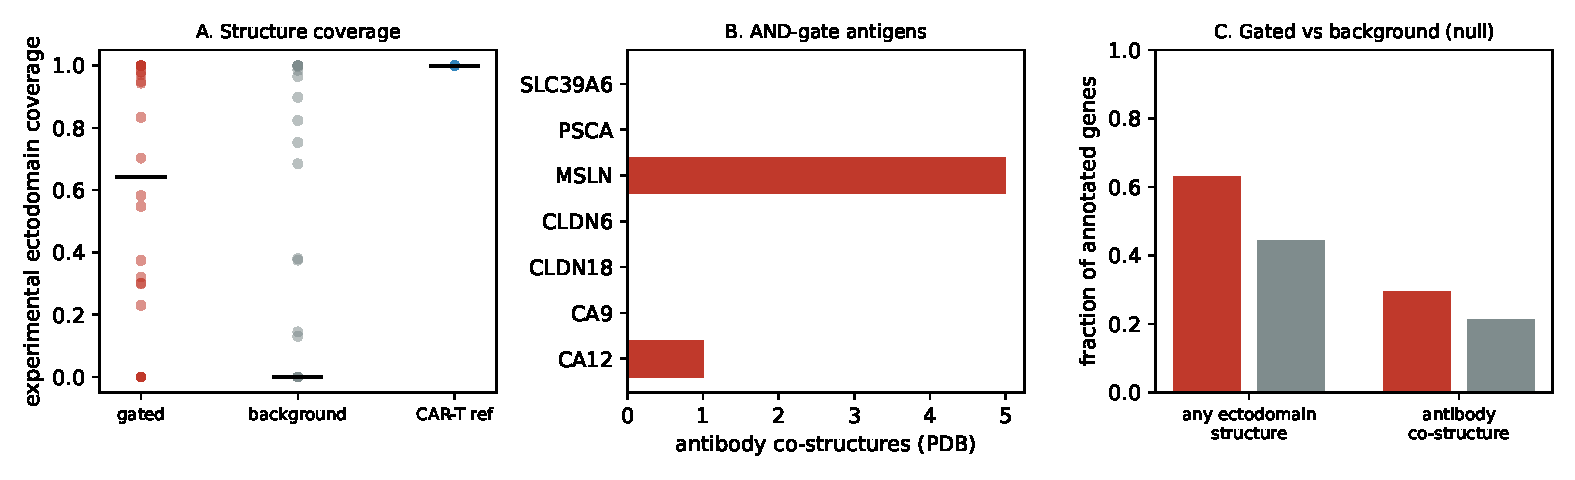
\includegraphics[width=\linewidth]{figs/fig_epitope.pdf}
\caption{A: experimental ectodomain coverage per gene (bars = medians). B:
antibody co-structures for the AND-gate antigens. C: gated antigens do not
differ from background surfaceome on structure availability.}\label{fig:epitope}
\end{figure}
